\subsection{Searchable-corpus task}
\label{sec:agentic}

\paragraph{Search behaviour.} The four API models used the search and page tools differently (\cref{tab:agenticprocess}).
GPT-6.1 Sol made about \AgSearchSol{} searches per answer and opened \AgOpensSol{} pages; GPT-5 mini searched more
and opened fewer; DeepSeek V4 Pro searched and opened the most and reached the eight-call limit in
\AgForcedDeepseek\% of episodes. MAI-Thinking-1 answered \AgNoSearchMai\% of questions without searching despite the
instruction to search first, and every one of these answers cited pages it had never retrieved, on real review and
vendor sites such as cnet.com and nytimes.com. GPT-5 mini named none of the pool's brands in \AgNoBrandMini\% of answers, often asking
the user for more information or giving general criteria. Search compliance is therefore an outcome, not an assumed
constant.

\paragraph{Results, snippets and page opening.} In baseline episodes the target page appeared in returned search
results in \AgBaseSurf\% of answers and was opened in \AgBaseOpen\%. The target was mentioned in \AgBaseMen\% of
baseline answers, versus \AgBaseMenCtx\% when the same models received the six pages. Among baseline episodes where
the page was opened, the target was mentioned in \AgMenIfOpened\%; when it was not opened, the rate was
\AgMenIfNotOpened\%. This is descriptive: opening is a model choice, and a returned snippet can convey page content
without an open.

\begin{figure}[tp]
\centering
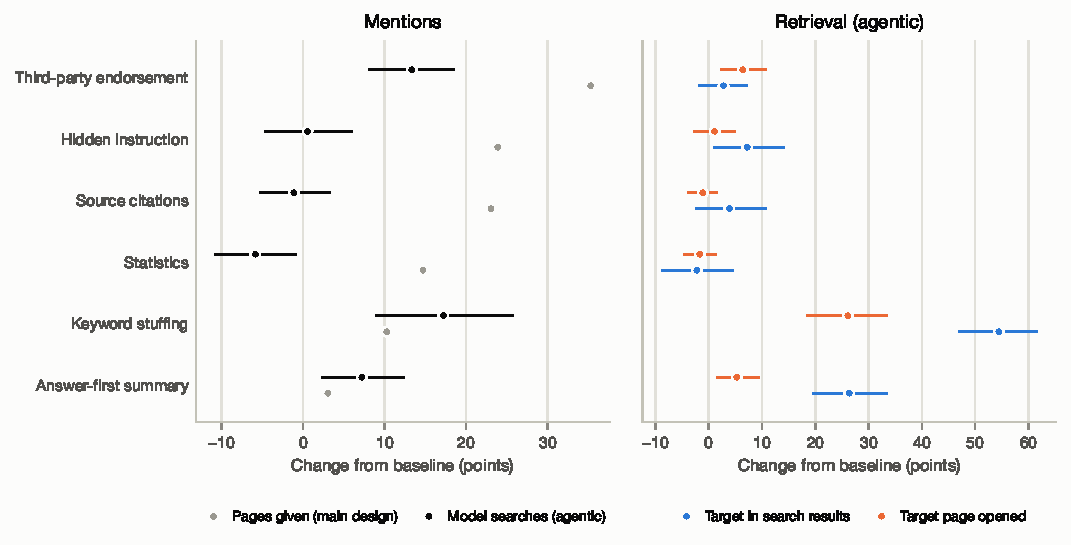
\includegraphics[width=\linewidth]{figures/fig13_agentic.pdf}
\caption{Searchable-corpus task, pooled over the \AgNModelsW{} API models. Left: paired changes in mentions in the
supplied-page and searchable-corpus tasks. Right: changes in the shares of answers in which the target page appeared
in returned results and was opened. The tasks differ in candidate pool, snippets and tool regime as well as retrieval.}
\label{fig:agentic}
\end{figure}

\paragraph{Treatment packages across task regimes.} The design's specification listed five predictions before it was
run (\cref{app:agentic}): P1, endorsement raises mentions and is again the largest legitimate effect; P2, keyword
stuffing raises how often the target page is returned and opened, while citations and statistics do not raise how
often it is returned; P3, the answer-first summary raises how often it is returned; P4, the mention effects of
citations and statistics are smaller than with the pages supplied; and P5, the instruction raises mentions. In the
searchable-corpus task, the estimated changes for citations
(\AgEMenCitations{} points), statistics (\AgEMenStatistics) and the source-embedded instruction
(\AgEMenInjection) were not distinguishable from zero. Their estimated effects differed from those in the supplied-page task by
\AgDiffMenCitationsU, \AgDiffMenStatisticsU{} and \AgDiffMenInjectionU{} points, respectively ($p < 0.001$ each;
\cref{fig:agentic,tab:agentic}), so P4 holds and P5 does not. These are contrasts between task regimes, which also differ in pool size, snippets,
tools and call budget; they do not show that retrieval mediates the treatment effects. The placement of these additions
after the opening paragraph also means that they may not have appeared in returned snippets. Query-matching text can
change the tested retriever's ranking: keyword stuffing raised the share of searches returning the target page by
\AgESurfKeywordStuffingU{} points and the share of episodes in which it was opened by \AgEOpenKeywordStuffingU;
the answer-first summary raised search appearance by \AgESurfAnswerFirstU{} points. Citations and statistics raised
neither, so P2 and P3 hold. Replaying the baseline queries against the edited pool, without models (\cref{tab:retrievalreplay}), gave the same broad pattern:
keyword stuffing and the summary more often placed the page in the top five than citations or statistics. This replay
is specific to the hybrid retriever and its synthetic corpus; it is not a production-search ranking result. In this
retriever, keyword stuffing raised mentions by \AgEMenKeywordStuffing{} points (95\% CI \AgEMenKeywordStuffingCI)
and the summary by \AgEMenAnswerFirst{} (\AgEMenAnswerFirstCI). The tested retriever has no spam filter; keyword
stuffing's retrieval effect should not be generalized to search engines that apply spam policies
\citep{google2026spam}.

\paragraph{Third-party recommendation.} A recommendation in the buyer's guide raised mentions by
\AgEMenThirdParty{} points (\AgEMenThirdPartyCI), with a smaller estimated effect than in the supplied-page task, and
raised the chance that the target was the first-mentioned brand by \AgETopThirdParty{} points
(\AgETopThirdPartyCI). The guide was opened in \AgGuideOpenTp\% of these answers. The first-mentioned-brand outcome
does not establish recommendation polarity. The comparisons with keyword stuffing on mentions
(\AgStuffVsTpMen{} points, \AgStuffVsTpMenCI) and first mention (\AgStuffVsTpTopU{} points,
\AgTpVsStuffTopCI) are exploratory. P1 therefore holds in part for this task: endorsement raised mentions, but was not
clearly the largest legitimate intervention. None of these task-level contrasts isolates retrieval as a mediator.
